\documentclass[10pt]{beamer}
\usepackage{graphicx}
\usepackage {mathtools}
%\usepackage{subfig}
\usepackage{subcaption}

\usetheme{CambridgeUS}
\usecolortheme{dolphin}

% set colors
\definecolor{myNewColorA}{RGB}{126,12,110}
\definecolor{myNewColorB}{RGB}{165,85,154}
\definecolor{myNewColorC}{RGB}{204,158,197}
\setbeamercolor*{palette primary}{bg=myNewColorC}
\setbeamercolor*{palette secondary}{bg=myNewColorB, fg = white}
\setbeamercolor*{palette tertiary}{bg=myNewColorA, fg = white}
\setbeamercolor*{titlelike}{fg=myNewColorA}
\setbeamercolor*{title}{bg=myNewColorA, fg = white}
\setbeamercolor*{item}{fg=myNewColorA}
\setbeamercolor*{caption name}{fg=myNewColorA}
\usefonttheme{professionalfonts}
\usepackage{natbib}
\usepackage{hyperref}
%------------------------------------------------------------
\titlegraphic{
\includegraphics[height=1.5cm]{vu_logo.png}}

\setbeamerfont{title}{size=\large}
\setbeamerfont{subtitle}{size=\small}
\setbeamerfont{author}{size=\small}
\setbeamerfont{date}{size=\small}
\setbeamerfont{institute}{size=\small}
\title[Vilnius University]{Flanker Task EEG functional data hypothesis testing}
\author {Jonas Adomaitis \and Tomas Giedraitis \and Gedas Beržinskas}

\institute{ Vilnius University

Faculty of Mathematics and Informatics}
\date[28.04.2026]

%------------------------------------------------------------
%This block of commands puts the table of contents at the
%beginning of each section and highlights the current section:
%\AtBeginSection[]
%{
%  \begin{frame}
%    \frametitle{Contents}
%    \tableofcontents[currentsection]
%  \end{frame}
%}
\AtBeginSection[]{
  \begin{frame}
  \vfill
  \centering
  \begin{beamercolorbox}[sep=8pt,center,shadow=true,rounded=true]{title}
    \usebeamerfont{title}\insertsectionhead\par%
  \end{beamercolorbox}
  \vfill
  \end{frame}
}
%------------------------------------------------------------

\begin{document}

%The next statement creates the title page.
\frame{\titlepage}
\begin{frame}
\frametitle{Contents}
\tableofcontents
\end{frame}
%------------------------------------------------------------
\section{Introduction}

\begin{frame}{Introduction}

  \begin{itemize}
        \item In this part of the project we test whether the functional EEG response curves during a Flanker task differ significantly between individuals with ADHD symptoms (n=12) and without (n=39).
    \end{itemize}

\begin{align*}
H_0 &: \mu_{\text{ADHD}}(t) = \mu_{\text{non-ADHD}}(t), \quad \forall \, t \in [-0.2, \, 0.8] \\
H_1 &: \mu_{\text{ADHD}}(t) \neq \mu_{\text{non-ADHD}}(t), \quad \text{for some } t
\end{align*}


\end{frame}

\section{Group Comparison}

\begin{frame}{Group Comparison}

    \centering
    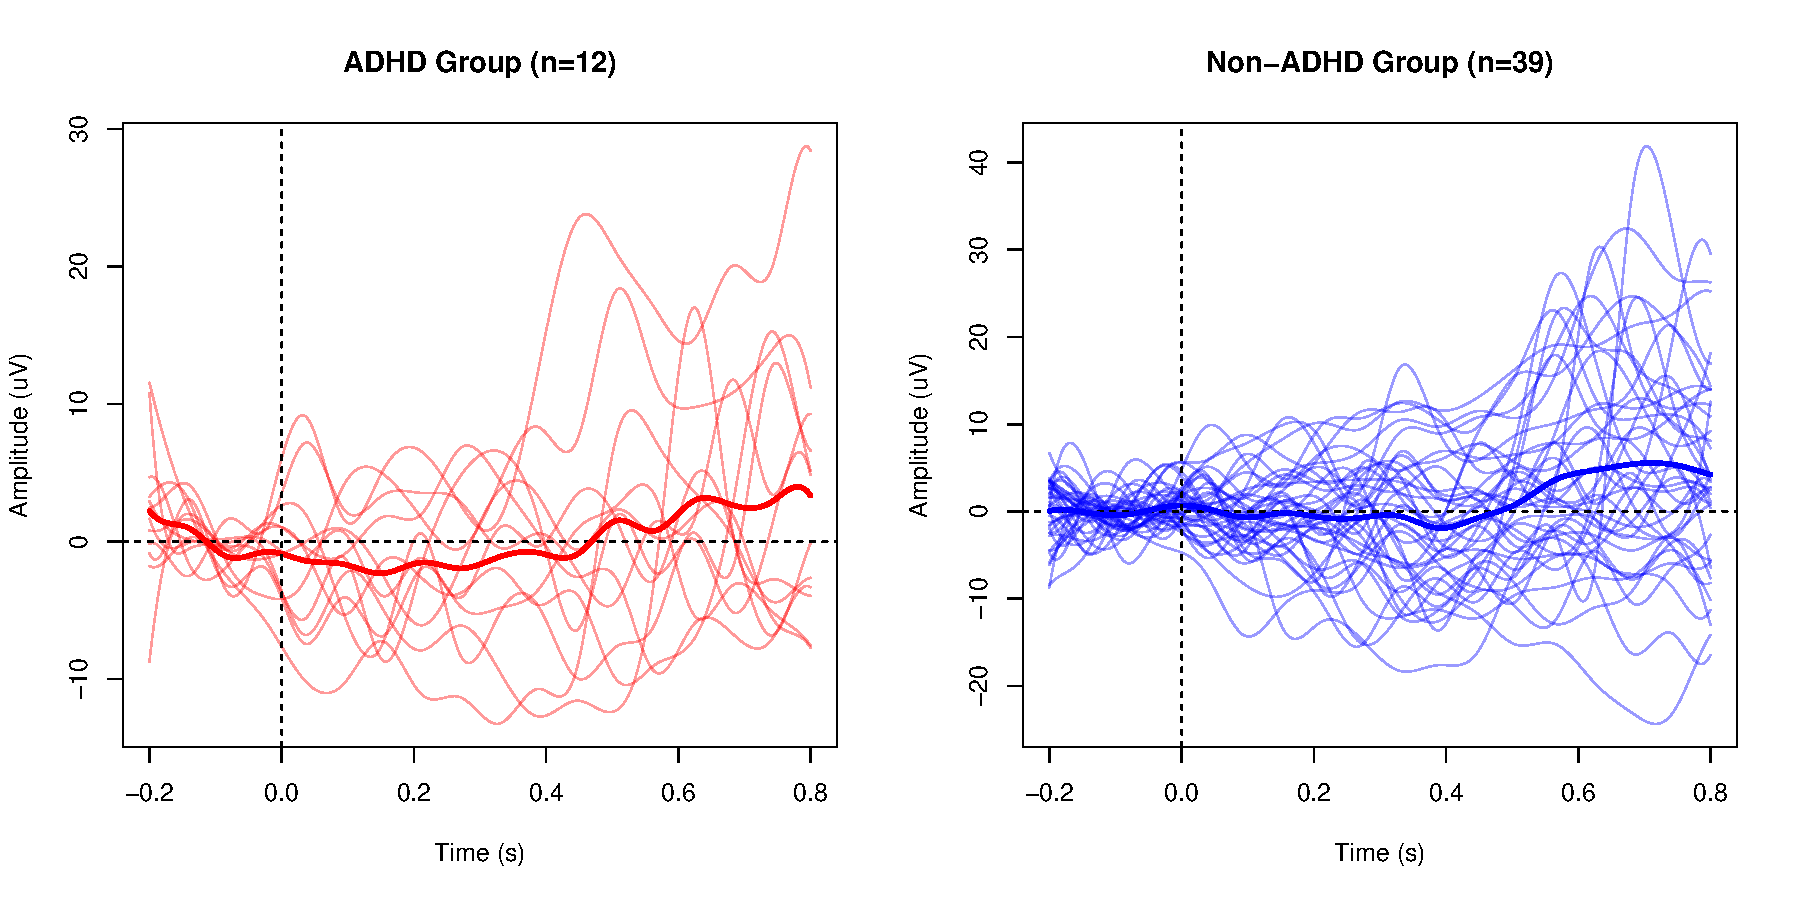
\includegraphics[width=1\textwidth]{HT_01_group_comparison.pdf}

\end{frame}

\section{Mean Curves}



\begin{frame}{Mean Curves}

    \centering
    
\includegraphics[width=1\textwidth]{HT_02_mean_comparison.pdf}

\end{frame}


\section{Hypothesis testing}

\begin{frame}{Pointwise Z-test}

    \centering
    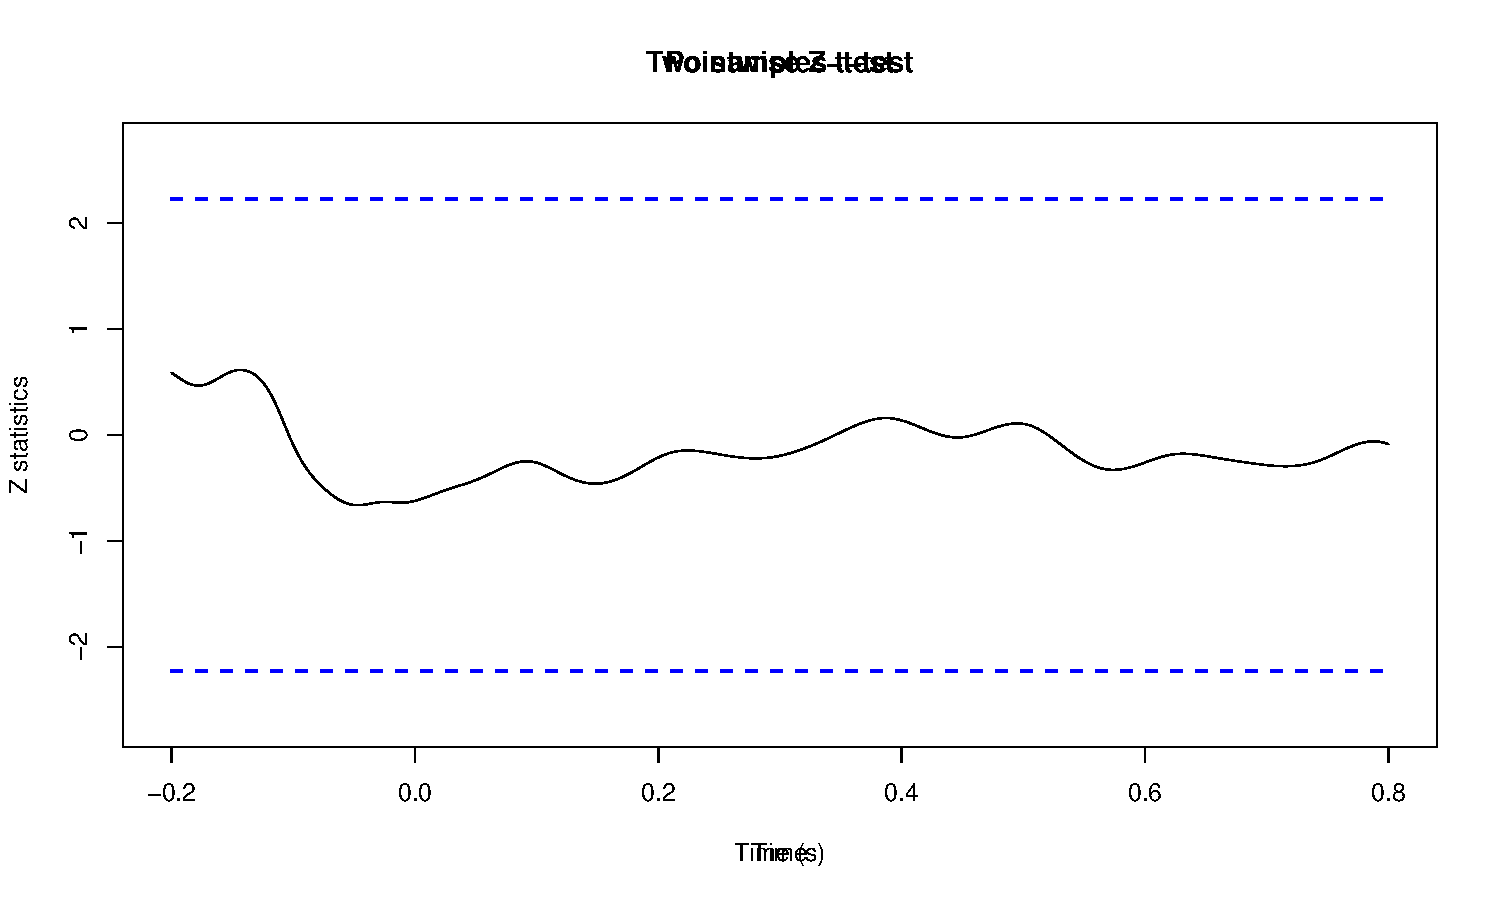
\includegraphics[width=1\textwidth]{HT_03_pointwise_Ztest.pdf}

\end{frame}


%--------------------------------------------------------------------------------
\begin{frame}{L2-norm Test}

The L2-norm test measures the total integrated squared difference between the two group mean curves:
$$T_{L^2} = \frac{nm}{n+m} \int \left[\bar{x}(t) - \bar{y}(t)\right]^2 dt$$

\vspace{0.3cm}

\begin{table}[h]
\centering
\begin{tabular}{l c c}
\hline
\textbf{Method} & \textbf{Statistic} & \textbf{p-value} \\
\hline
Naive ($\chi^2$ approximation) & 10882.89 & 1.0000 \\
Bootstrap (500 replications) & 10882.89 & 0.7260 \\
\hline
\end{tabular}
\end{table}

\vspace{0.3cm}

{\small Both methods yield large p-values ($p > 0.05$), indicating no significant global difference between the ADHD and non-ADHD mean curves.}

\end{frame}


\begin{frame}{F-type Test}

The F-type test normalizes the L2 statistic by the trace of the covariance operator:
$$F = \frac{T_{L^2}}{\mathrm{tr}(\hat{\Sigma})}$$

\vspace{0.3cm}

\begin{table}[h]
\centering
\begin{tabular}{l c c}
\hline
\textbf{Method} & \textbf{Statistic} & \textbf{p-value} \\
\hline
Naive ($F$ approximation) & 0.0818 & 1.0000 \\
Bootstrap (500 replications) & 0.0818 & 0.7140 \\
\hline
\end{tabular}
\end{table}

\vspace{0.3cm}

{\small The F-type test accounts for the covariance structure of the data. Large p-values ($p > 0.05$) confirm no significant difference between the two groups.}

\end{frame}



%--------------------------------------------------------------------------------



\begin{frame}{Permutation Test}

    \centering
    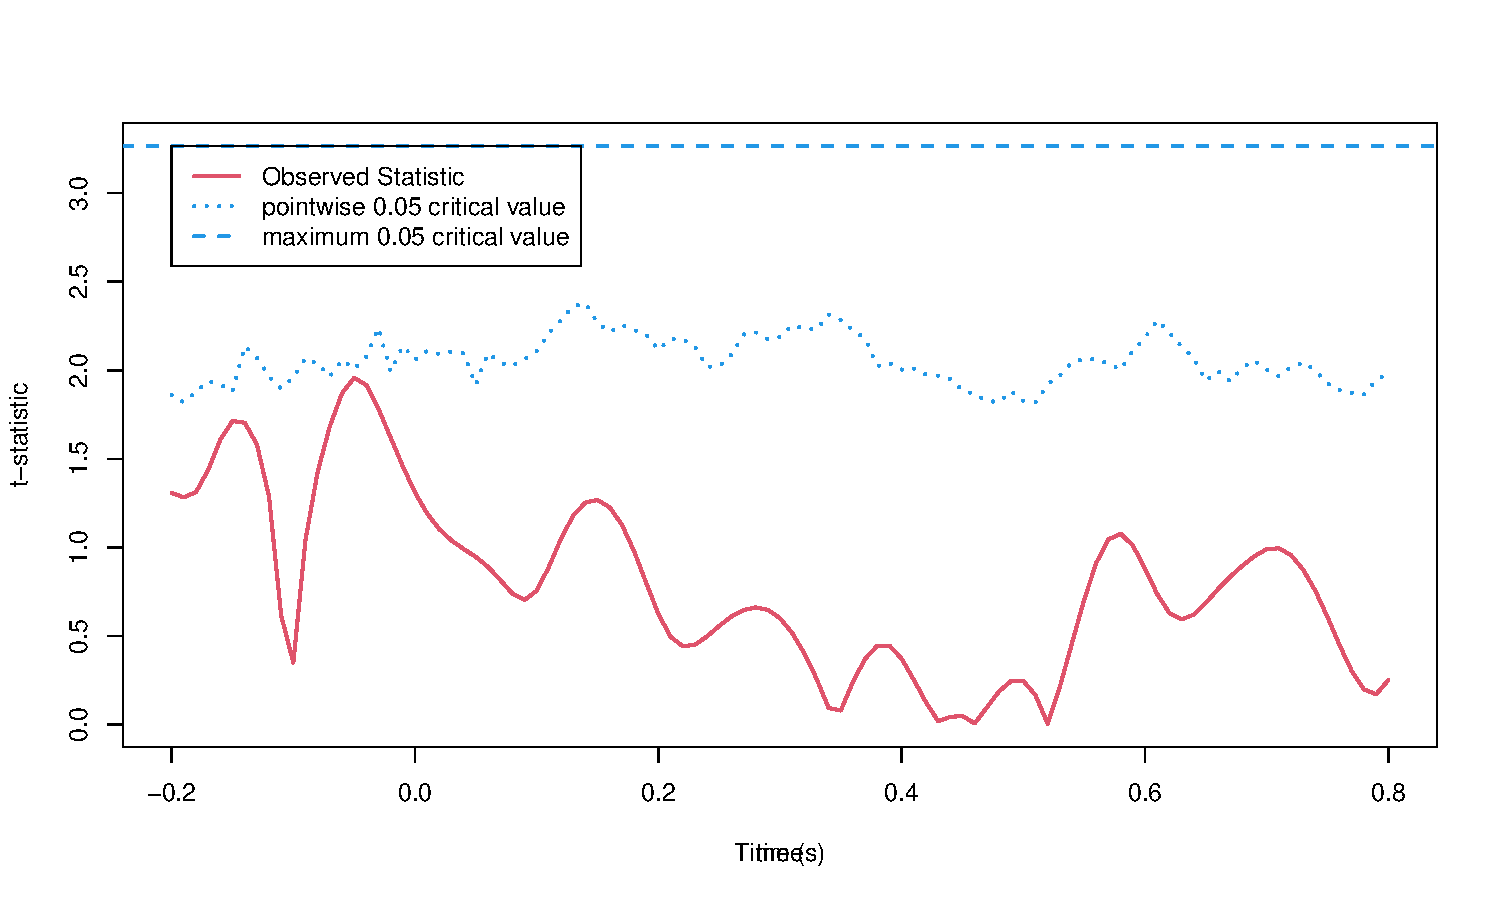
\includegraphics[width=1\textwidth]{HT_04_permutation_test.pdf}

\end{frame}

\section{Summary}
\begin{frame}{Summary}

\begin{table}[h]
\centering
\begin{tabular}{l c}
\hline
\textbf{Test} & \textbf{p-value} \\
\hline
Pointwise Z-test (max $|Z|$ = 0.66) & -- \\
L2-norm test (naive) & 1.0000 \\
L2-norm test (bootstrap) & 0.7260 \\
F-type test (naive) & 1.0000 \\
F-type test (bootstrap) & 0.7140 \\
Permutation test & 0.5250 \\
\hline
\end{tabular}
\end{table}

\vspace{0.3cm}

\textbf{Conclusion:} All tests fail to reject $H_0$ at $\alpha = 0.05$. There is no significant difference between the EEG response curves of individuals with and without ADHD symptoms during the Flanker task at channel FC1.

\vspace{0.3cm}

{\small This may be due to the small ADHD group size (n=12), the use of a single EEG channel, or the nature of the ADHD classification.}

\end{frame}





\section*{Acknowledgements}
\begin{frame}
\textcolor{myNewColorA}{\Huge{\centerline{Thank you for your time!}}}

\end{frame}




\end{document}

